% Source PDF page 249 (printed p. 235)
原始问题（5.25），其中 $f_0,\ldots,f_m$ 凸，并假设Slater条件成立：存在 $\widetilde x\in\relint D$，使 $f_i(\widetilde x)<0$，$i=1,\ldots,m$，且 $A\widetilde x=b$。为简化证明，再作两个假设：第一，$D$ 的内部非空（因而 $\relint D=\operatorname{int}D$）；第二，$\rank A=p$。假设 $p^\star$ 有限。（由于存在可行点，$p^\star$ 只能是 $-\infty$ 或有限值；若 $p^\star=-\infty$，弱对偶给出 $d^\star=-\infty$。）

容易证明，若原问题凸，（5.37）定义的集合 $\mathcal A$ 就是凸的。再定义另一个凸集
\[
\mathcal B=\{(0,0,s)\in\R^m\times\R^p\times\R\mid s<p^\star\}.
\]
$\mathcal A$ 与 $\mathcal B$ 不相交。事实上，若 $(u,v,t)\in\mathcal A\cap\mathcal B$，由 $(u,v,t)\in\mathcal B$，有 $u=0$、$v=0$、$t<p^\star$；由 $(u,v,t)\in\mathcal A$，存在 $x$，使 $f_i(x)\le0$，$i=1,\ldots,m$，$Ax-b=0$，且 $f_0(x)\le t<p^\star$。但 $p^\star$ 是原始问题最优值，因此不可能出现这种情况。

由§2.5.1的分离超平面定理，存在 $(\widetilde\lambda,\widetilde\nu,\mu)\ne0$ 和 $\alpha$，使得
\begin{equation}
(u,v,t)\in\mathcal A\ \Longrightarrow\
\widetilde\lambda^\T u+\widetilde\nu^\T v+\mu t\ge\alpha,\tag{5.39}
\end{equation}
以及
\begin{equation}
(u,v,t)\in\mathcal B\ \Longrightarrow\
\widetilde\lambda^\T u+\widetilde\nu^\T v+\mu t\le\alpha.\tag{5.40}
\end{equation}
由（5.39）得到 $\widetilde\lambda\succeq0$、$\mu\ge0$。（否则 $\widetilde\lambda^\T u+\mu t$ 在 $\mathcal A$ 上无下界，与（5.39）矛盾。）条件（5.40）仅意味着，对所有 $t<p^\star$，有 $\mu t\le\alpha$，因而 $\mu p^\star\le\alpha$。结合（5.39），可知对于任意 $x\in D$，
\begin{equation}
\sum_{i=1}^m\widetilde\lambda_i f_i(x)
+\widetilde\nu^\T(Ax-b)+\mu f_0(x)\ge\alpha\ge\mu p^\star.\tag{5.41}
\end{equation}
设 $\mu>0$。把（5.41）除以 $\mu$，得到对所有 $x\in D$，
\[
L(x,\widetilde\lambda/\mu,\widetilde\nu/\mu)\ge p^\star.
\]
对 $x$ 最小化，便得 $g(\lambda,\nu)\ge p^\star$，其中定义
\[
\lambda=\widetilde\lambda/\mu,\qquad \nu=\widetilde\nu/\mu.
\]
弱对偶给出 $g(\lambda,\nu)\le p^\star$，所以实际上 $g(\lambda,\nu)=p^\star$。这证明，至少当 $\mu>0$ 时，强对偶成立且对偶最优值能达到。

再考虑 $\mu=0$。由（5.41）可知，对于所有 $x\in D$，
\begin{equation}
\sum_{i=1}^m\widetilde\lambda_i f_i(x)+\widetilde\nu^\T(Ax-b)\ge0.\tag{5.42}
\end{equation}
将其用于满足Slater条件的 $\widetilde x$，得到
\[
\sum_{i=1}^m\widetilde\lambda_i f_i(\widetilde x)\ge0.
\]

% Source PDF page 250 (printed p. 236)
\begin{figure}[htbp]\centering
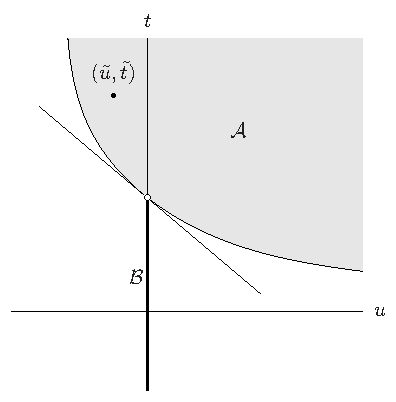
\includegraphics[width=.55\linewidth]{figures/ch05-fig06.pdf}
\caption*{图5.6\quad 满足Slater约束资格的凸问题的强对偶证明示意图。阴影区域为 $\mathcal A$，粗竖线段为 $\mathcal B$，不包含以小空心圆表示的点 $(0,p^\star)$。两个集合凸且不相交，因此可由超平面分离。Slater约束资格保证任意分离超平面都是非竖直的，因为它必须从点 $(\widetilde u,\widetilde t)=(f_1(\widetilde x),f_0(\widetilde x))$ 左侧通过，其中 $\widetilde x$ 严格可行。}
\end{figure}
由于 $f_i(\widetilde x)<0$ 且 $\widetilde\lambda_i\ge0$，可知 $\widetilde\lambda=0$。由 $(\widetilde\lambda,\widetilde\nu,\mu)\ne0$、$\widetilde\lambda=0$ 和 $\mu=0$，可知 $\widetilde\nu\ne0$。于是（5.42）说明，对所有 $x\in D$，$\widetilde\nu^\T(Ax-b)\ge0$。但 $\widetilde x$ 满足 $\widetilde\nu^\T(A\widetilde x-b)=0$，且 $\widetilde x\in\operatorname{int}D$，所以除非 $A^\T\widetilde\nu=0$，否则 $D$ 中必有点满足 $\widetilde\nu^\T(Ax-b)<0$。这当然与假设 $\rank A=p$ 矛盾。

图5.6用只有一个不等式约束的简单问题说明证明背后的几何思想。分离 $\mathcal A$ 和 $\mathcal B$ 的超平面在 $(0,p^\star)$ 处支撑 $\mathcal A$。Slater约束资格用来证明该超平面必非竖直（即法向量可写为 $(\lambda^\star,1)$）。（一个只有一个不等式约束但强对偶失败的简单凸问题，见习题5.21。）

\subsection{多准则解释}
不含等式约束的问题
\begin{equation}
\begin{array}{ll}\text{最小化}&f_0(x)\\
\text{约束为}&f_i(x)\le0,\quad i=1,\ldots,m\end{array}\tag{5.43}
\end{equation}
的拉格朗日对偶，与无约束多准则问题的标量化方法之间存在自然联系。

% Source PDF page 251 (printed p. 237)
这里的多准则问题为
\begin{equation}
\text{最小化（相对于 $\R_+^{m+1}$）}\quad
F(x)=(f_1(x),\ldots,f_m(x),f_0(x))\tag{5.44}
\end{equation}
（见§4.7.4）。标量化时，选择正向量 $\widetilde\lambda$，并最小化标量函数 $\widetilde\lambda^\T F(x)$；任意最小点都保证是Pareto最优的。将 $\widetilde\lambda$ 乘正数不影响最小点，因此不失一般性，可取 $\widetilde\lambda=(\lambda,1)$。于是标量化所最小化的函数是
\[
\widetilde\lambda^\T F(x)=f_0(x)+\sum_{i=1}^m\lambda_i f_i(x),
\]
它恰好是问题（5.43）的拉格朗日函数。

为证明凸多准则问题的每个Pareto最优点，都在某个非负权向量 $\widetilde\lambda$ 下最小化 $\widetilde\lambda^\T F(x)$，我们曾考虑（4.62）定义的集合 $\mathcal A$，
\[
\mathcal A=\{t\in\R^{m+1}\mid\exists x\in D,\ f_i(x)\le t_i,\ i=0,\ldots,m\}.
\]
它与拉格朗日对偶中（5.37）定义的集合 $\mathcal A$ 完全相同。这里同样通过任意Pareto最优点处的支撑超平面来构造所需的权向量。在多准则优化中，权向量各分量表示目标函数之间的相对权重。当把对应于 $f_0$ 的最后一个分量固定为1时，其他权重就表示相对于 $f_0$ 的代价，即相对于目标的代价。

\section{鞍点解释}
本节给出拉格朗日对偶的几种解释。后续内容不会用到本节材料。

\subsection{弱对偶与强对偶的最大—最小刻画}
可以用更对称的形式表示原始和对偶优化问题。为简化讨论，假设没有等式约束；这些结果很容易推广到含等式约束的情况。

首先注意，
\[
\begin{aligned}
\sup_{\lambda\succeq0}L(x,\lambda)
&=\sup_{\lambda\succeq0}\left(f_0(x)+\sum_{i=1}^m\lambda_i f_i(x)\right)\\
&=\begin{cases}
f_0(x)&f_i(x)\le0,\quad i=1,\ldots,m,\\
\infty&\text{其他情形}.
\end{cases}
\end{aligned}
\]

% Source PDF page 252 (printed p. 238)
事实上，若 $x$ 不可行，且某个 $i$ 满足 $f_i(x)>0$，取 $\lambda_j=0$（$j\ne i$），再令 $\lambda_i\to\infty$，就有 $\sup_{\lambda\succeq0}L(x,\lambda)=\infty$。另一方面，若 $f_i(x)\le0$，$i=1,\ldots,m$，则 $\lambda$ 的最优选择是零，因而 $\sup_{\lambda\succeq0}L(x,\lambda)=f_0(x)$。这说明原始问题的最优值可写为
\[
p^\star=\inf_x\sup_{\lambda\succeq0}L(x,\lambda).
\]
由对偶函数定义，还有
\[
d^\star=\sup_{\lambda\succeq0}\inf_xL(x,\lambda).
\]
因此，弱对偶可表示为不等式
\begin{equation}
\sup_{\lambda\succeq0}\inf_xL(x,\lambda)
\le\inf_x\sup_{\lambda\succeq0}L(x,\lambda),\tag{5.45}
\end{equation}
强对偶则表示为等式
\[
\sup_{\lambda\succeq0}\inf_xL(x,\lambda)
=\inf_x\sup_{\lambda\succeq0}L(x,\lambda).
\]
强对偶意味着，关于 $x$ 的最小化和关于 $\lambda\succeq0$ 的最大化可以交换次序，而不改变结果。

事实上，不等式（5.45）不依赖于 $L$ 的任何性质：对任意 $f:\R^n\times\R^m\to\R$（以及任意 $W\subseteq\R^n$、$Z\subseteq\R^m$），有
\begin{equation}
\sup_{z\in Z}\inf_{w\in W}f(w,z)
\le\inf_{w\in W}\sup_{z\in Z}f(w,z).\tag{5.46}
\end{equation}
这一一般不等式称为\emph{最大—最小不等式}。当等号成立，即
\begin{equation}
\sup_{z\in Z}\inf_{w\in W}f(w,z)
=\inf_{w\in W}\sup_{z\in Z}f(w,z),\tag{5.47}
\end{equation}
就称 $f$（以及 $W,Z$）满足\emph{强最大—最小性质}或\emph{鞍点性质}。强最大—最小性质当然只在特殊情形下成立，例如 $f:\R^n\times\R^m\to\R$ 是一个具有强对偶的问题的拉格朗日函数，$W=\R^n$、$Z=\R_+^m$ 时。

\subsection{鞍点解释}
若 $\widetilde w\in W$、$\widetilde z\in Z$ 满足对所有 $w\in W$、$z\in Z$，
\[
f(\widetilde w,z)\le f(\widetilde w,\widetilde z)\le f(w,\widetilde z),
\]
就称 $(\widetilde w,\widetilde z)$ 为 $f$（以及 $W,Z$）的\emph{鞍点}。换言之，$\widetilde w$ 在 $w\in W$ 上最小化 $f(w,\widetilde z)$，$\widetilde z$ 在 $z\in Z$ 上最大化 $f(\widetilde w,z)$：
\[
f(\widetilde w,\widetilde z)=\inf_{w\in W}f(w,\widetilde z),\qquad
f(\widetilde w,\widetilde z)=\sup_{z\in Z}f(\widetilde w,z).
\]

% Source PDF page 253 (printed p. 239)
由此可知强最大—最小性质（5.47）成立，且共同值为 $f(\widetilde w,\widetilde z)$。

回到拉格朗日对偶：若一个强对偶成立的问题中，$x^\star$ 和 $\lambda^\star$ 分别为原始和对偶最优点，它们就构成拉格朗日函数的一个鞍点。反之也成立：若 $(x,\lambda)$ 是拉格朗日函数的鞍点，那么 $x$ 是原始最优点，$\lambda$ 是对偶最优点，且最优对偶间隙为零。

\subsection{博弈解释}
可以用一个连续零和博弈解释最大—最小不等式（5.46）、最大—最小等式（5.47）和鞍点性质。若参与者1选择 $w\in W$，参与者2选择 $z\in Z$，则参与者1向参与者2支付 $f(w,z)$。因此参与者1希望最小化 $f$，参与者2则希望最大化 $f$。（之所以称为连续博弈，是因为选择是向量，而非离散选项。）

假设参与者1先选择，然后参与者2在获知参与者1的选择后再选择。参与者2希望最大化支付 $f(w,z)$，因此将选择 $z\in Z$ 使 $f(w,z)$ 最大。所得支付为 $\sup_{z\in Z}f(w,z)$，它依赖于参与者1的选择 $w$。（这里假设上确界能达到；若不能，最优支付可任意接近 $\sup_{z\in Z}f(w,z)$。）参与者1知道（或假定）参与者2将采取这个策略，因此选择 $w\in W$，使最坏情况下向参与者2的支付尽可能小。于是参与者1选择
\[
\argmin_{w\in W}\sup_{z\in Z}f(w,z),
\]
得到从参与者1向参与者2的支付
\[
\inf_{w\in W}\sup_{z\in Z}f(w,z).
\]

再假设行动次序颠倒：参与者2必须先选择 $z\in Z$，然后参与者1在知道 $z$ 的情况下选择 $w\in W$。类似地，若双方采取最优策略，参与者2应选择 $z\in Z$ 最大化 $\inf_{w\in W}f(w,z)$，从而得到从参与者1向参与者2的支付
\[
\sup_{z\in Z}\inf_{w\in W}f(w,z).
\]

最大—最小不等式（5.46）表达了一个直观事实：后行动对参与者更有利，更准确地说，在作选择前知道对手的选择更有利。换言之，若参与者1必须先选，参与者2得到的支付会更大。当鞍点性质（5.47）成立时，后行动就没有优势。

若 $(\widetilde w,\widetilde z)$ 是 $f$（以及 $W,Z$）的鞍点，便称它为博弈的\emph{解}；称 $\widetilde w$ 为参与者1的\emph{最优选择}或\emph{最优策略}，称 $\widetilde z$ 为参与者2的最优选择或最优策略。

% Source PDF page 254 (printed p. 240)
这时后行动没有优势。

现在考虑支付函数为拉格朗日函数、$W=\R^n$、$Z=\R_+^m$ 的特殊情形。此时参与者1选择原始变量 $x$，参与者2选择对偶变量 $\lambda\succeq0$。根据上面的论证，若参与者2必须先选，她的最优选择就是任意对偶最优的 $\lambda^\star$，由此得到支付 $d^\star$。反之，若参与者1必须先选，他的最优选择是任意原始最优的 $x^\star$，得到支付 $p^\star$。

问题的最优对偶间隙，恰好等于后行动的参与者所获得的优势，也就是在作选择前知道对手选择的优势。若强对偶成立，知道对手的选择对双方都不带来优势。

\subsection{价格或税收解释}
拉格朗日对偶有一个有趣的经济解释。设变量 $x$ 表示企业的运营方式，$f_0(x)$ 表示在 $x$ 下的运营成本，即 $-f_0(x)$ 是运营状态 $x$ 下的利润（例如以美元计）。每个约束 $f_i(x)\le0$ 表示某种限制，例如资源限制（仓储空间、劳动力等）或监管限制（如环保限制）。在遵守限制的同时实现利润最大的运营状态，可通过求解问题
\[
\begin{array}{ll}\text{最小化}&f_0(x)\\
\text{约束为}&f_i(x)\le0,\quad i=1,\ldots,m\end{array}
\]
得到。最优利润为 $-p^\star$。

再设想第二种情形：允许违反限制，但需要支付一笔与违反程度（由 $f_i$ 衡量）成线性关系的额外成本。因此，企业针对第 $i$ 个限制或约束支付 $\lambda_i f_i(x)$。对不紧的约束，也会向企业付款；若 $f_i(x)<0$，则 $\lambda_i f_i(x)$ 表示向企业支付的一笔钱。系数 $\lambda_i$ 可理解为违反 $f_i(x)\le0$ 的价格，单位是每单位违反量（由 $f_i$ 衡量）所需的美元数。企业还能以同一价格出售第 $i$ 个约束的“未用”部分。假设 $\lambda_i\ge0$，即企业要为违反约束付款（若约束不紧，则获得收入）。

例如，原问题第一个约束 $f_1(x)\le0$ 表示仓储空间限制（以平方米计）。在新安排下，企业可以按每平方米 $\lambda_1$ 美元的价格租入额外仓储空间，也可以同样的价格出租未使用空间。

运营状态为 $x$、约束价格为 $\lambda_i$ 时，企业总成本为
$L(x,\lambda)=f_0(x)+\sum_{i=1}^m\lambda_i f_i(x)$。企业显然会选择最小化总成本 $L(x,\lambda)$ 的运营方式，得到成本 $g(\lambda)$。因此，对偶函数表示企业最优成本关于约束价格向量 $\lambda$ 的函数。最优对偶值 $d^\star$ 就是企业在最不利价格组合下的最优成本。

% Source PDF page 255 (printed p. 241)
利用这个解释，弱对偶可表述为：在第二种情形中（允许买卖约束违反量），即使价格最不利，企业的最优成本也不大于原情形（约束不得违反）下的成本。这是明显的：若 $x^\star$ 是第一种情形的最优解，则第二种情形下采用 $x^\star$ 的运营成本会低于 $f_0(x^\star)$，因为不紧的约束还可能带来一些收入。因此，最优对偶间隙就是企业因获准付费违反约束（并因约束不紧而得到款项）所获得的最小可能优势。

现在假设强对偶成立，且对偶最优值能达到。对偶最优的 $\lambda^\star$ 可解释为一组价格：在这组价格下，允许企业付费违反约束（或因约束不紧而收款）并不带来优势。因此，对偶最优的 $\lambda^\star$ 有时称为原问题的一组\emph{影子价格}。

\section{最优性条件}
提醒读者，除非明确说明，我们并不假设问题（5.1）是凸的。

\subsection{次优性证书与停止准则}
若能找到对偶可行的 $(\lambda,\nu)$，就能确定原始问题最优值的下界：$p^\star\ge g(\lambda,\nu)$。因此，对偶可行点 $(\lambda,\nu)$ 提供 $p^\star\ge g(\lambda,\nu)$ 的一个证明或\emph{证书}。强对偶意味着存在任意精确的证书。

不必知道 $p^\star$ 的精确值，对偶可行点就能为给定可行点的次优程度提供界。事实上，若 $x$ 原始可行、$(\lambda,\nu)$ 对偶可行，则
\[
f_0(x)-p^\star\le f_0(x)-g(\lambda,\nu).
\]
这特别说明，$x$ 是 $\epsilon$-次优的，其中 $\epsilon=f_0(x)-g(\lambda,\nu)$。（同时也说明 $(\lambda,\nu)$ 是对偶问题的 $\epsilon$-次优点。）

把原始和对偶目标之间的差
\[
f_0(x)-g(\lambda,\nu)
\]
称为原始可行点 $x$ 与对偶可行点 $(\lambda,\nu)$ 对应的\emph{对偶间隙}。原始—对偶可行点对 $x,(\lambda,\nu)$ 将原始（及对偶）问题的最优值定位在区间内：
\[
p^\star\in[g(\lambda,\nu),f_0(x)],\qquad
d^\star\in[g(\lambda,\nu),f_0(x)],
\]
区间宽度就是对偶间隙。

若原始—对偶可行点对 $x,(\lambda,\nu)$ 的对偶间隙为零，即 $f_0(x)=g(\lambda,\nu)$，则 $x$ 是原始最优点，$(\lambda,\nu)$ 是对偶最优点。可以把 $(\lambda,\nu)$ 看作证明 $x$ 最优的证书。

% Source PDF page 256 (printed p. 242)
类似地，也可把 $x$ 看作证明 $(\lambda,\nu)$ 对偶最优的证书。

在优化算法中，这些观察可用于给出非启发式停止准则。假设算法产生原始可行序列 $x^{(k)}$ 和对偶可行序列 $(\lambda^{(k)},\nu^{(k)})$，$k=1,2,\ldots$，给定所需绝对精度 $\epsilon_{\mathrm{abs}}>0$。那么停止准则（即终止算法的条件）
\[
f_0(x^{(k)})-g(\lambda^{(k)},\nu^{(k)})\le\epsilon_{\mathrm{abs}}
\]
保证算法终止时，$x^{(k)}$ 是 $\epsilon_{\mathrm{abs}}$-次优的。事实上，$(\lambda^{(k)},\nu^{(k)})$ 就是证明这一点的证书。（当然，要使此方法对任意小容差 $\epsilon_{\mathrm{abs}}$ 有效，必须有强对偶。）

类似条件可以保证给定相对精度 $\epsilon_{\mathrm{rel}}>0$。若
\[
g(\lambda^{(k)},\nu^{(k)})>0,\qquad
\frac{f_0(x^{(k)})-g(\lambda^{(k)},\nu^{(k)})}
{g(\lambda^{(k)},\nu^{(k)})}\le\epsilon_{\mathrm{rel}},
\]
或
\[
f_0(x^{(k)})<0,\qquad
\frac{f_0(x^{(k)})-g(\lambda^{(k)},\nu^{(k)})}
{-f_0(x^{(k)})}\le\epsilon_{\mathrm{rel}},
\]
则 $p^\star\ne0$，且相对误差
\[
\frac{f_0(x^{(k)})-p^\star}{|p^\star|}
\]
保证不大于 $\epsilon_{\mathrm{rel}}$。

\subsection{互补松弛}
假设原始和对偶最优值都能达到且相等（特别地，强对偶成立）。设 $x^\star$ 是原始最优点，$(\lambda^\star,\nu^\star)$ 是对偶最优点。这意味着
\[
\begin{aligned}
f_0(x^\star)&=g(\lambda^\star,\nu^\star)\\
&=\inf_x\left(f_0(x)+\sum_{i=1}^m\lambda_i^\star f_i(x)
+\sum_{i=1}^p\nu_i^\star h_i(x)\right)\\
&\le f_0(x^\star)+\sum_{i=1}^m\lambda_i^\star f_i(x^\star)
+\sum_{i=1}^p\nu_i^\star h_i(x^\star)\\
&\le f_0(x^\star).
\end{aligned}
\]
第一行表示最优对偶间隙为零，第二行是对偶函数的定义。第三行源于拉格朗日函数关于 $x$ 的下确界不大于它在 $x=x^\star$ 的取值。最后一个不等式源于 $\lambda_i^\star\ge0$、$f_i(x^\star)\le0$，$i=1,\ldots,m$，及 $h_i(x^\star)=0$，$i=1,\ldots,p$。因此，不等式链中的两个不等式都必须取等号。

% Source PDF page 257 (printed p. 243)
由此能得出几个有趣结论。例如，第三行不等式取等号说明 $x^\star$ 关于 $x$ 最小化 $L(x,\lambda^\star,\nu^\star)$。（拉格朗日函数 $L(x,\lambda^\star,\nu^\star)$ 还可能有其他最小点；$x^\star$ 只是其中之一。）

另一个重要结论是
\[
\sum_{i=1}^m\lambda_i^\star f_i(x^\star)=0.
\]
由于和式中每项都非正，可知
\begin{equation}
\lambda_i^\star f_i(x^\star)=0,\quad i=1,\ldots,m.\tag{5.48}
\end{equation}
这一条件称为\emph{互补松弛}；当强对偶成立时，它对任意原始最优 $x^\star$ 和任意对偶最优 $(\lambda^\star,\nu^\star)$ 都成立。互补松弛可写为
\[
\lambda_i^\star>0\ \Longrightarrow\ f_i(x^\star)=0,
\]
或等价地，
\[
f_i(x^\star)<0\ \Longrightarrow\ \lambda_i^\star=0.
\]
粗略地说，除非第 $i$ 个约束在最优点处是活跃的，否则第 $i$ 个最优拉格朗日乘子为零。

\subsection{KKT最优性条件}
现在假设 $f_0,\ldots,f_m,h_1,\ldots,h_p$ 可微（因此其定义域为开集），但仍未对凸性作假设。

\subsubsection*{非凸问题的KKT条件}
同上，设 $x^\star$ 和 $(\lambda^\star,\nu^\star)$ 是任意一对对偶间隙为零的原始、对偶最优点。由于 $x^\star$ 关于 $x$ 最小化 $L(x,\lambda^\star,\nu^\star)$，其梯度必在 $x^\star$ 处为零，即
\[
\nabla f_0(x^\star)+\sum_{i=1}^m\lambda_i^\star\nabla f_i(x^\star)
+\sum_{i=1}^p\nu_i^\star\nabla h_i(x^\star)=0.
\]
因此有
\begin{equation}
\begin{gathered}
f_i(x^\star)\le0,\quad i=1,\ldots,m,\\
h_i(x^\star)=0,\quad i=1,\ldots,p,\\
\lambda_i^\star\ge0,\quad i=1,\ldots,m,\\
\lambda_i^\star f_i(x^\star)=0,\quad i=1,\ldots,m,\\
\nabla f_0(x^\star)+\sum_{i=1}^m\lambda_i^\star\nabla f_i(x^\star)
+\sum_{i=1}^p\nu_i^\star\nabla h_i(x^\star)=0,
\end{gathered}\tag{5.49}
\end{equation}
这些条件称为\emph{Karush--Kuhn--Tucker（KKT）条件}。

综上，对于目标函数和约束函数都可微、且强对偶成立的任意优化问题，任意一对原始和对偶最优点都必须满足KKT条件（5.49）。

% Source PDF page 258 (printed p. 244)
\subsubsection*{凸问题的KKT条件}
当原始问题凸时，KKT条件也是原始和对偶最优的充分条件。换言之，若 $f_i$ 凸、$h_i$ 仿射，且 $\widetilde x,\widetilde\lambda,\widetilde\nu$ 满足KKT条件
\[
\begin{gathered}
f_i(\widetilde x)\le0,\quad i=1,\ldots,m,\\
h_i(\widetilde x)=0,\quad i=1,\ldots,p,\\
\widetilde\lambda_i\ge0,\quad i=1,\ldots,m,\\
\widetilde\lambda_i f_i(\widetilde x)=0,\quad i=1,\ldots,m,\\
\nabla f_0(\widetilde x)+\sum_{i=1}^m\widetilde\lambda_i\nabla f_i(\widetilde x)
+\sum_{i=1}^p\widetilde\nu_i\nabla h_i(\widetilde x)=0,
\end{gathered}
\]
则 $\widetilde x$、$(\widetilde\lambda,\widetilde\nu)$ 分别是原始和对偶最优点，且对偶间隙为零。

为说明这一点，注意前两个条件表示 $\widetilde x$ 原始可行。由于 $\widetilde\lambda_i\ge0$，$L(x,\widetilde\lambda,\widetilde\nu)$ 关于 $x$ 凸；最后一个KKT条件表示它关于 $x$ 的梯度在 $x=\widetilde x$ 处为零，因此 $\widetilde x$ 关于 $x$ 最小化 $L(x,\widetilde\lambda,\widetilde\nu)$。由此得到
\[
\begin{aligned}
g(\widetilde\lambda,\widetilde\nu)&=L(\widetilde x,\widetilde\lambda,\widetilde\nu)\\
&=f_0(\widetilde x)+\sum_{i=1}^m\widetilde\lambda_i f_i(\widetilde x)
+\sum_{i=1}^p\widetilde\nu_i h_i(\widetilde x)\\
&=f_0(\widetilde x),
\end{aligned}
\]
最后一步利用了 $h_i(\widetilde x)=0$ 和 $\widetilde\lambda_i f_i(\widetilde x)=0$。这说明 $\widetilde x$ 和 $(\widetilde\lambda,\widetilde\nu)$ 的对偶间隙为零，因此分别原始最优和对偶最优。综上，对于任意目标和约束函数均可微的凸优化问题，满足KKT条件的点就是原始和对偶最优点，且对偶间隙为零。

若目标和约束函数均可微的凸优化问题满足Slater条件，那么KKT条件给出最优性的充要条件：Slater条件蕴含最优对偶间隙为零且对偶最优值能达到，所以 $x$ 最优，当且仅当存在 $(\lambda,\nu)$，与 $x$ 一起满足KKT条件。

KKT条件在优化中起重要作用。少数特殊情形下，可以解析地求解KKT条件（从而求解优化问题）。更一般地，许多凸优化算法本来就是，或可以解释为，求解KKT条件的方法。

\begin{origexample}{5.1}
\emph{等式约束凸二次最小化。}考虑问题
\begin{equation}
\begin{array}{ll}\text{最小化}&(1/2)x^\T Px+q^\T x+r\\
\text{约束为}&Ax=b,\end{array}\tag{5.50}
\end{equation}
其中 $P\in\mathbf S_+^n$。该问题的KKT条件为
\[
Ax^\star=b,\qquad Px^\star+q+A^\T\nu^\star=0,
\]
可写为
\[
\begin{bmatrix}P&A^\T\\A&0\end{bmatrix}
\begin{bmatrix}x^\star\\\nu^\star\end{bmatrix}
=\begin{bmatrix}-q\\b\end{bmatrix}.
\]
